\documentclass[dvipdfmx,b5paper,papersize]{jsarticle}
\usepackage{amsthm}
\usepackage{amsmath}
\usepackage{amssymb}
\usepackage{amsfonts}
\usepackage{tikz}


\pagestyle{empty}
\theoremstyle{definition}
\newtheorem{thm}{Thm.}
\newtheorem{prop}[thm]{Prop.}
\newtheorem{cor}[thm]{Cor.}
\newtheorem{defi}[thm]{Def.}
\newtheorem{lem}[thm]{Lem.}
\newtheorem{rem}[thm]{Rem.}
\newtheorem{ex}[thm]{Ex.}
\renewcommand{\abstractname}{}
\renewcommand{\labelenumi}{(\alabic{enumi})}
\title{quasi-coherent algebraとrelative spectrum}
\author{荒井勇人(36)\footnote{東大数学科新3年.twitter:@alskdjfhg9.記事の内容とは関係ないですが,IT関係のバイトを探しています.}}
\date{}


\begin{document}
\maketitle

\begin{abstract}
  環に対するaffine schemeを一般化した概念として,quasi-coherent algebraに対応するrelative spectrumというものを紹介する.大雑把にいうと,scheme $S$上のある種の環のsheaf $\cal{A}$から,$\cal{A}$(に近いsheaf)をstructure sheaf に持つようなscheme ${\rm Spec}{\cal{A}}$を構成する.さらにこれがいくつかの普遍性を満たすことを示す.

\end{abstract}

\section{導入}
環$A$に対しaffine scheme ${\rm Spec}A$が定義され,$A$はstructure sheafという形で${\rm Spec}A$上の関数と思えるのであった(\cite{ハーツホーン}など).そして${\rm Spec}A$はadjoint
\[
  {\rm Hom}_{\bf Sch}(X,{\rm Spec}A) \xrightarrow{\sim} {\rm Hom}_{\bf Ring}(A,\Gamma(X,{\cal{O}}_X))
\]
によって特徴付けられる(\cite{Gortz} Prop.3.4).この記事では\cite{Bosch}および\cite{stacks_project}に従い,scheme $S$上のquasi-coherent ${\cal{O}}_S$-algebraという種類のsheaf $\cal{A}$についてその$S$上のrelative spectrum ${\rm Spec}{\cal{A}}$を定義し,類似のadjointを示すことでaffine schemeの一般化になっていることをみる.また応用として,米田埋め込みと組み合わせてfiber productの計算に利用する.

環は可換で$1$をもち,環準同型は$1$を保ち,$0\neq 1$とする.


\section{${\cal{O}}_{X}$\it{-modules}}
環上の加群に対応する概念として,scheme $X$上の${\cal{O}}_{X}$-moduleを定義する.
\begin{defi}[${\cal{O}}_X$-module]
  scheme $(X,{\cal{O}}_X)$に対して,${\cal{O}}_X$-module $\cal{F}$とは$X$上のAbel群のsheaf $\cal{F}$とsheafの射${\cal{O}}_X \times \cal{F} \to \cal{F}$の組であって,各開集合$U \subset X$について${\cal{O}}_X(U)\times{\cal{F}}(U)\to{\cal{F}}(U)$
  が${\cal{F}}(U)$に${\cal{O}}_X(U)$
  加群の構造を与えるようなもののことである.

  また,${\cal{O}}_X$-moduleの射とはsheafの射$\cal{F} \to \cal{G}$であって下図を可換にするもの,

  \[
    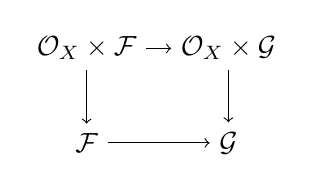
\begin{tikzpicture}[auto,->]
      \node (a) at (0,1.2) {${\cal{O}}_X \times \cal{F}$}; \node (x) at (1.8,1.2) {${\cal{O}}_X \times \cal{G}$};
      \node (b) at (0,0) {$\cal{F}$}; \node (y) at (1.8,0) {$\cal{G}$};
      \draw (a) -- node {$\scriptstyle $} (x);
      \draw (x) -- node {$\scriptstyle $} (y);
      \draw (a) -- node[swap] {$\scriptstyle $} (b);
      \draw (b) -- node[swap] {$\scriptstyle $} (y);
    \end{tikzpicture}
  \]
  つまり各開集合$U \subset X$について${\cal{F}}(U) \to {\cal{G}}(U)$が${{\cal{O}}_X}(U)$加群の射となるようなもののことである.

  %%$S$上の$\cal{O}_{S}$-moduleのなす圏を$\cal{O}_S$-Modとかく.
\end{defi}


\begin{thm}
  ${\cal{O}}_X$-moduleの圏${\cal{O}}_X$-ModはAbel圏である.
\end{thm}

\begin{proof}
  $X$上のAbel群のsheafのなすAbel圏におけるKer,Coker,直和などが${\cal{O}}_X$-ModにおけるKer,Coker,直和になっている.

\end{proof}
${\cal{O}}_{X}$-moduleの基本的な例として,$X={\rm Spec}A$のとき$A$加群$M$から作られる${\cal{O}}_{X}$-module ${\tilde M}$がある.
\begin{defi}[associated module]
  $A$を環とし,$X={\rm Spec}A$とする.このとき$A$加群$M$に対し${\cal{O}}_X$-module ${\tilde M}$を,$f \in A$に対して
  \[
    D(f) \longmapsto M_f=M \otimes _A A_f
  \]
  を満たすものとして定める(これはaffine schemeの構成と同様の証明によりwell-definedとなる).これを$M$に付随する${\cal{O}}_X$-module (${\cal{O}}_X$-module associated to $M$)という\footnote{特に$M=A$のとき,${\tilde A}={\cal{O}}_X$である.}.

  また,$A$加群の射$\varphi :M \to N$に対し,${\cal{O}}_X$-moduleの射${\tilde \varphi :\tilde M \to \tilde N}$を,局所化による射
  \[
    \tilde \varphi (D(f)) = \varphi _f : M_f \to N_f
  \]
  によって定める.
  これにより関手$A\mathchar`-Mod \to {\cal{O}}_{X}\mathchar`-Mod$が定まる.
\end{defi}

\begin{prop}
  $A$を環,$X={\rm Spec}A$とする.$A$加群$M$と${\cal{O}}_X$-module $\cal{F}$について,自然同型
  \[
    {\rm Hom}_A(M,{\cal{F}}(X)) \longrightarrow {\rm Hom}_{{\cal{O}}_X}(\tilde M,\cal{F}),\hspace{15pt} \varphi \longmapsto \tilde \varphi
  \]
  がある.特に関手$M \mapsto \tilde M$は大域切断のleft adjointである.
\end{prop}

\begin{proof}
inverseが大域切断$\psi \longmapsto \psi(X)$で与えられることを示す.$\psi :\tilde M \to \cal{F}$を任意に取ったとき$f \in A$に対して可換図式
\[
  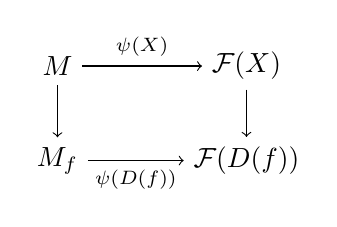
\begin{tikzpicture}[auto,->]
    \node (a) at (0,1.2) {$M$}; \node (x) at (2.4,1.2) {${\cal{F}}(X)$};
    \node (b) at (0,0) {$M_f$}; \node (y) at (2.4,0) {${\cal{F}}(D(f))$};
    \draw (a) -- node {$\scriptstyle \psi(X)$} (x);
    \draw (x) -- node {$\scriptstyle $} (y);
    \draw (a) -- node[swap] {$\scriptstyle $} (b);
    \draw (b) -- node[swap] {$\scriptstyle \psi(D(f))$} (y);
  \end{tikzpicture}
\]
を考える.${\cal{F}}(D(f))$は$A_f$加群だから,局所化の普遍性により$\psi(D(f))$は$\psi(X)$のみによって復元できる.よって大域切断がinverseである.自然性は明らか.
\end{proof}

\begin{defi}[quasi-coherent module]
  $X$をschemeとし,$\cal{F}$を${\cal{O}}_X$-moduleとする.全てのaffine open subscheme $U \subset X$に対して,${\cal{F}}|_U$がある${\cal{O}}_X(U)$加群$M_U$に付随する${\cal{O}}_X|_U$-moduleであるとき,$\cal{F}$はquasi-coherentであるという.以下q-coh.と略す.


\end{defi}

\begin{rem}\label{thm:q-coh.local}
  実は,q-coh.の定義において「全てのaffine open subschemeに対して」とする代わりに「$X$のあるaffine open covering $(U_i)_i$が存在して」としても同値である\footnote{\cite{Bosch}, \S 6.8, Thm.10.}.特にaffine scheme上ではq-coh.とassociated moduleの概念が一致する.
\end{rem}
\begin{rem}
  $\cal{F}$がq-coh. ${\cal{O}}_X$-moduleで,$U={\rm Spec}A \subset X$がaffine open subschemeなら,$f \in A$に対し
  \[
    {\cal{F}}(D(f))={\cal{F}}(U)_f
  \]
  が成り立つ.

\end{rem}

\section{${\cal{O}}_X${\it-module}の順像,逆像}
位相空間の間の連続写像によって,sheafの順像,逆像という演算が定義されadjointになっているのであった\footnote{\cite{Gortz}, \S 2.8など.}.ここでは${\cal{O}}_X$-moduleの順像,逆像を構成する.
\begin{defi}
  $R$を環,$X$,$Y$を位相空間とし,$f:X \longrightarrow Y$を連続写像,$\cal{F}$,$\cal{G}$をそれぞれ$X$,$Y$上の$R$加群のsheafとする.このとき$Y$上の$R$加群のsheaf
  \[
    V \longmapsto {\cal{F}}(f^{-1}(V)), \hspace{15pt} V \subset Y:open
  \]
  を$f_*{\cal{F}}$と書き,$\cal{F}$の$f$による順像(direct image)という.これにより自然に関手
  \[
    f_*:Sh(X,R\mathchar`-Mod) \longrightarrow Sh(Y,R\mathchar`-Mod)
  \]
  が定まる.

  また,$f_*$のleft adjointを
  \[
    f^{-1}:Sh(Y,R\mathchar`-Mod) \longrightarrow Sh(X,R\mathchar`-Mod)
  \]
  と書き,$f^{-1}\cal{G}$を$\cal{G}$の$f$による逆像(inverse image)という.
\end{defi}

\begin{defi}[${\cal{O}}_X$-moduleのテンソル積]
  $X$をschemeとし,$\cal{F}$,$\cal{G}$を${\cal{O}}_X$-moduleとする.presheaf
  \[
    U \longmapsto {\cal{F}}(U) \otimes_{{{\cal{O}}_X}(U)} {\cal{G}}(U), \hspace{15pt} U \subset X:open
  \]
  のsheafificationを${\cal{F}} \otimes_{{\cal{O}}_X} {\cal{G}}$と書き,${\cal{F}}$と${\cal{G}}$の${\cal{O}}_X$上のテンソル積という.これは自然に${\cal{O}}_X$-moduleになる.
\end{defi}
詳細は省略するが,このテンソル積は普通のテンソル積に関係した普遍性(係数拡大など)に似た形の普遍性を満たすことがわかる.これを用いて${\cal{O}}_X$-moduleの逆像を構成する.
\begin{prop}\label{thm:inverse}
  $X$,$Y$をschemeとし,$f:X \longrightarrow Y$をschemeの射,$\cal{F},\cal{G}$をそれぞれ${\cal{O}}_X,{\cal{O}}_Y$-moduleとする.$f^{-1}\cal{G}$は自然に$f^{-1}{\cal{O}}_Y$-moduleになり,また$f$による$f^{-1}{\cal{O}}_Y \longrightarrow {\cal{O}}_X$により${\cal{O}}_X$を$f^{-1}{\cal{O}}_Y$-moduleとみて
  \[
    f^*{\cal{G}}=f^{-1}{\cal{G}} \otimes_{f^{-1}{{\cal{O}}_Y}} {\cal{O}}_X
  \]
  とおく.
  このとき自然同型
  \[
    {\rm Hom}_{{\cal{O}}_X}(f^*{\cal{G}},{\cal{F}}) \xrightarrow{\sim} {\rm Hom}_{{\cal{O}}_Y}({\cal{G}},f_*{{\cal{F}}})
  \]
  がある.
\end{prop}
\begin{proof}
  Abel群のsheafとしてのadjointによる自然同型
  \[
    {\rm Hom}_{X}(f^{-1}{\cal{G}},{\cal{F}}) \xrightarrow{\sim} {\rm Hom}_{Y}({\cal{G}},f_*{{\cal{F}}})
  \]
  は,自然同型
  \[
    {\rm Hom}_{f^{-1}{\cal{O}}_Y}(f^*{\cal{G}},{\cal{F}}) \xrightarrow{\sim} {\rm Hom}_{{\cal{O}}_Y}({\cal{G}},f_*{{\cal{F}}})
    \]
  を誘導する.
  また,テンソル積による係数拡大の普遍性とsheafificationの普遍性を使うと,自然同型
  \[
    {\rm Hom}_{f^{-1}{\cal{O}}_Y}(f^{-1}{\cal{G}},{\cal{F}}) \xrightarrow{\sim} {\rm Hom}_{{\cal{O}}_Y}(f^{-1}{\cal{G}} \otimes_{f^{-1}{{\cal{O}}_Y}} {\cal{O}}_X,{\cal{F}})
  \]
  がある.これらよりわかる.
\end{proof}
\begin{defi}[${\cal{O}}_X$-moduleの順像,逆像]
  $X$,$Y$をschemeとし,$f:X \longrightarrow Y$をschemeの射,$\cal{F}$,$\cal{G}$をそれぞれ${\cal{O}}_X,{\cal{O}}_Y$-moduleとする.${\cal{F}}$の$f$による順像(direct image)とは,Abel群のsheafとしての順像$f_*{{\cal{F}}}$のことである.また,${\cal{G}}$の$f$による逆像(inverse image)とは{\rm Prop.\ref{thm:inverse}}で構成した$f^*{\cal{G}}$のことと定める.
\end{defi}
次の命題より,affineな場合順像,逆像は係数制限,係数拡大によってかけることがわかる.特にq-coh.が逆像で保たれることに注意する.
\begin{prop}\label{thm:associated}
  $X={\rm Spec}{A},Y={\rm Spec}{B}$をaffine scheme,$f:X \to Y$を$\sigma:B \to A$に対応する射とする.また,$F$を$A$加群,$G$を$B$加群とする.このとき
  \[
    f_*({\tilde F})={\widetilde {F_{/B}}}, \hspace{15pt} f^*({\tilde G})={\widetilde {G \otimes_B A}}
  \]
  である.ここで${F_{/B}}$は$\sigma:B \to A$による係数制限である.
\end{prop}
\begin{proof}
  $g \in B$とする.
  \[
    f_*({\tilde F})(D(g))={\tilde F}(D(\sigma(g)))=F\otimes_A A_{\sigma(g)}
  \]
  だが,$A_{\sigma(g)}=A\otimes_B B_g$だから
  \[
    F\otimes_A A_{\sigma(g)}=F\otimes_A (A\otimes_B B_g)=F_{/B}\otimes_B B_g
  \]
  である.よって$f_*({\tilde F})={\widetilde {F_{/B}}}$である.

  また任意の${\cal{O}}_X$-module ${\cal{F}}$について,$F={\cal{F}}(X)$とおくと
  \[
    {\rm Hom}_{{\cal{O}}_X}(f^*{\tilde G},{\cal{F}})\cong {\rm Hom}_{{\cal{O}}_Y}({\tilde G},f_*{{\cal{F}}})
  \]
  で,係数拡大およびsheafの大域切断に伴うadjointより
  \[
    {\rm Hom}_{{\cal{O}}_Y}({\tilde G},f_*{{\cal{F}}})\cong {\rm Hom}_{B}(G,F_{/B})\cong {\rm Hom}_{A}(G\otimes_B A,F)\cong {\rm Hom}_{{\cal{O}}_X}({\widetilde {G \otimes_B A}},{\cal{F}})
  \]
  が成り立つ.よって米田の補題より$f^*({\tilde G})={\widetilde {G \otimes_B A}}$である.
\end{proof}
\begin{cor}\label{thm:invese_q-coh.}
  $f:X\to Y$をschemeの射とし,$\cal{G}$をq-coh. ${\cal{O}}_Y$-moduleとする.このとき$f^*{\cal{G}}$はq-coh. ${\cal{O}}_X$-moduleである.
\end{cor}
\begin{proof}
  $Y$のaffine open subscheme $V$に対し,$f(U) \subset V$となるような$X$のaffine open subscheme $U$をとる.このとき$f^*$の構成より
  \[
    (f^*({\cal{G}}))|_U=f^*({\cal{G}}|_V)
  \]
  である.そしてこのような$U,V$を全て考えると$U$たちは$X$を覆う.よってProp.\ref{thm:associated}とRem.\ref{thm:q-coh.local}より$f^*({\cal{G}})$はq-coh.である.

\end{proof}




\section{${\cal{O}}_{X}$\it{-algebras}}
環$R$に対する$R$代数に対応する概念として,${\cal{O}}_{X}$-algebraを定義する.
\begin{defi}[${\cal{O}}_X$-algebra]
  scheme $(X,{\cal{O}}_X)$に対して,${\cal{O}}_X$-algebra $\cal{A}$とは,$X$上の環のsheaf $\cal{A}$とsheafの射${\cal{O}}_X \to \cal{A}$の組のことである.

  また,${\cal{O}}_X$-algebraの射とは,sheafの射$\cal{A} \to \cal{B}$であって下図を可換にするもののこと,
  \[
    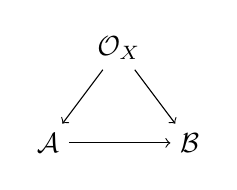
\begin{tikzpicture}[auto,->]
      \node (a) at (0.9,1.2) {${\cal{O}}_X$};
      \node (b) at (0,0) {$\cal{A}$}; \node (y) at (1.8,0) {$\cal{B}$};


      \draw (a) -- node[swap] {$\scriptstyle $} (b);
      \draw (a) -- node[swap] {$\scriptstyle $} (y);
      \draw (b) -- node[swap] {$\scriptstyle $} (y);
  \end{tikzpicture}
  \]

  つまり各開集合$U \subset X$について${\cal{A}}(U) \to {\cal{B}}(U)$が${{\cal{O}}_X}(U)$代数の射となるようなもののことである.
\end{defi}
${\cal{O}}_X$-algebraに対してもq-coh.が定義される.
\begin{defi}[quasi-coherent algebra]
  $(X,{\cal{O}}_X)$をschemeとする.quasi-coherent ${\cal{O}}_X$-algebraとは,${\cal{O}}_X$-moduleとしてq-coh.な${\cal{O}}_X$-algebraのことである.

\end{defi}

\begin{ex}[q-coh. polynomial algebra]
  $S$をschemeとする.このとき環のpresheaf
  \[
    U \longmapsto {\cal{O}}_S(U)[t_1,\dots ,t_n]
  \]
  のsheafificationを${\cal{O}}_S[t_1,\dots ,t_n]$と書く.これはq-coh. ${\cal{O}}_S$-algebraである.実際$U \subset S$をaffine openとすると,$U$に制限すればpresheafの時点で${\widetilde{{\cal{O}}_S(U)}}$と同型である.
\end{ex}

ここまでの準備のもとで,q-coh. ${\cal{O}}_S$-algebra $\cal{A}$のrelative spectrum ${\rm Spec}{\cal{A}}$を構成する.モチベーションは,「${\cal{A}}$に近い」structure sheafをもつ自然な$S$-schemeを定義したいというものである.そこで$S$のaffine open subscheme $U$について${\rm Spec}{\cal{A}}(U)$を考え,sheafの制限射に対応するaffine schemeの射を使って${\rm Spec}{\cal{A}}(U)$たちを貼り合わせる,といった感じのことをする.
\begin{thm}[relative spectrum]\label{thm:glueing}
  $S$をscheme,$(U_i)_i$を$S$のaffine open covering,$\cal{A}$をq-coh. ${\cal{O}}_S$-algebraとする.

  \[
    \pi_i:X_i={\rm Spec}{\cal{A}}(U_i) \longrightarrow U_i
  \]
  を$\sigma_i:{\cal{O}}_{S}(U_i) \to {\cal{A}}(U_i)$に対応するaffine schemeの射とする.このときschemeの同型
  \[
    \pi_{i}^{-1}(U_i\cap U_j) \xrightarrow{\sim} \pi_{j}^{-1}(U_i\cap U_j)
  \]
  があり,これによって$X_i$と$\pi_i$を貼り合わせて
  \[
    \pi:X \longrightarrow S
  \]
  ができる.この$X$を${\rm Spec}{\cal{A}}$と書き,$\cal{A}$の$S$上のrelative spectrumという.
\end{thm}
\begin{proof}
  まず,各$U_{ij\lambda}$が$U_i,U_j$両方の中でbasic open($D(g)$型の開集合)であり
  \[
    U_i \cap U_j=\bigcup_{\lambda}U_{ij\lambda}
  \]
  となるような$S$の開集合族$(U_{ij\lambda})_\lamda$が取れる.\footnote{\cite{Gortz}, Lem.3.3より.}$g \in {\cal{O}}_S(U_i)$によって$U_{ij\lambda}=D(g) \subset U_i$とかけているとする.$\cal{A}$がq-coh.だから${\cal{A}}(U_i)_g={\cal{A}}(U_{ij\lambda})$が成り立つ.よって
  \[
  \pi_{i}^{-1}(U_{ij \lambda})=D(\sigma_i(g))\cong {\rm Spec}{\cal{A}}(U_i)_g={\rm Spec}{\cal{A}}(U_{ij\lambda})
  \]
  となり,同型
  \[
    \pi_{i}^{-1}(U_{ij\lambda}) \xrightarrow{\sim} \pi_{j}^{-1}(U_{ij\lambda})
  \]
  がある.$U_{ij\lambda'}=D(g')$とおくと$U_{ij\lambda} \cap U_{ij\lambda'}=D(gg')$だから,この射は同型
  \[
    \pi_{i}^{-1}(U_{ij\lambda} \cap U_{ij\lambda'}) \xrightarrow{\sim} \pi_{j}^{-1}(U_{ij\lambda} \cap U_{ij\lambda'})
  \]
  を誘導する.よってschemeの射の貼り合わせにより同型
  \[
    \varphi_{ji}:\pi_{i}^{-1}(U_i\cap U_j) \xrightarrow{\sim} \pi_{j}^{-1}(U_i\cap U_j)
  \]
  ができる.作り方より,この同型はcocycle condition $\varphi_{ki}=\varphi_{kj} \circ \varphi_{ji}$を満たすから,$X_i$たちはglueing lemma(\cite{ハーツホーン}演習問題2.12,\cite{Gortz} Prop.3.10)により貼り合ってscheme $X$を作る.

  さらに
  \[
    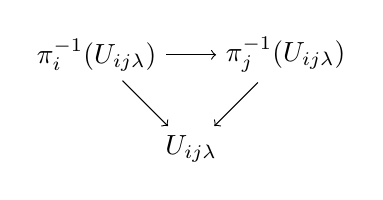
\begin{tikzpicture}[auto,->]
      \node (a) at (0,1.2) {$\pi_{i}^{-1}(U_{ij\lambda})$}; \node (x) at (2.4,1.2) {$\pi_{j}^{-1}(U_{ij\lambda})$};
      \node (b) at (1.2,0) {$U_{ij\lambda}$};
      \draw (a) -- node {$\scriptstyle $} (x);

      \draw (a) -- node[swap] {$\scriptstyle $} (b);
      \draw (x) -- node[swap] {$\scriptstyle $} (b);
    \end{tikzpicture}
  \]
  の可換性より
  \[
    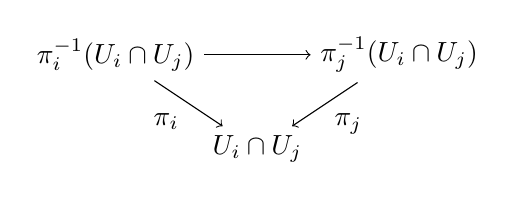
\begin{tikzpicture}[auto,->]
      \node (a) at (0,1.2) {$\pi_{i}^{-1}(U_i \cap U_j)$}; \node (x) at (3.6,1.2) {$\pi_{j}^{-1}(U_i \cap U_j)$};
      \node (b) at (1.8,0) {$U_i \cap U_j$};
      \draw (a) -- node {$\scriptstyle $} (x);

      \draw (a) -- node[swap] {$\pi_i$} (b);
      \draw (x) -- node {$\pi_j$} (b);
    \end{tikzpicture}
  \]
  の可換性がわかる.よってglueingの普遍性により$\pi_i$は貼り合って
  \[
    \pi:X \longrightarrow S
  \]
  ができる.
\end{proof}

\begin{cor}\label{thm:iso}
  {\rm Thm.\ref{thm:glueing}}の状況で,glueingによる射
  \[
    {\rm Spec}{\cal{A}}(U_i)=X_i \longrightarrow X={\rm Spec}{\cal{A}}
  \]
  は$S$-schemeとしての同型
  \[
    {\rm Spec}{\cal{A}}(U_i)\cong \pi^{-1}(U_i)
  \]
  を誘導する.
\end{cor}
\begin{proof}
  glueing lemmaの証明における構成より従う.

\end{proof}

\begin{thm}\label{thm:univ}
  $S$-scheme $q:Y\to S$とq-coh. ${\cal{O}}_S$-algebra $\cal{A}$に対し,自然同型
  \[
    {\rm Hom}_{S}(Y,{\rm Spec}{\cal{A}}) \xrightarrow{\sim} {\rm Hom}_{{\cal{O}}_S}({\cal{A}},q_*{{\cal{O}}_Y})
  \]
  がある.
\end{thm}
\begin{proof}

  まず,${\cal{O}}_S$-algebraの同型${\cal{A}} \xrightarrow{\sim} \pi_*{\cal{O}}_{{\rm Spec}{\cal{A}}}$を作る.Thm.\ref{thm:glueing}の証明より同型
  \[
    {\cal{A}}|_{U_i} \cong
    \pi_{i,*}{\cal{O}}_{{\rm Spec}{\cal{A}}(U_i)}
  \]が,Cor.\ref{thm:iso}より同型
  \[
    \pi_{i,*}{\cal{O}}_{{\rm Spec}{\cal{A}}(U_i)} \cong \pi_*({\cal{O}}_{{\rm Spec}{\cal{A}}}|_{\pi^{-1}(U_i)})=(\pi_*{\cal{O}}_X)|_{U_i}
  \]
  がある.よって同型${\cal{A}}|_{U_i}\xrightarrow{\sim}(\pi_*{\cal{O}}_{{\rm Spec}{\cal{A}}})|_{U_i}$があり,これらは貼り合わさって${\cal{O}}_S$-algebraの同型
  \[
    {\cal{A}} \xrightarrow{\sim} \pi_*{\cal{O}}_{{\rm Spec}{\cal{A}}}
  \]
  を定める\footnote{すなわち,${\rm Spec}{\cal{A}}$のstructure sheafはほとんど$\cal{A}$そのものである.}.

  次に$f\in{\rm Hom}_{S}(Y,{\rm Spec}{\cal{A}})$とする.
  \[
    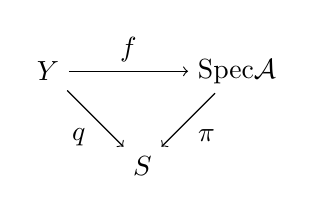
\begin{tikzpicture}[auto,->]
      \node (a) at (0,1.2) {$Y$}; \node (x) at (2.4,1.2) {${\rm Spec}{\cal{A}}$};
      \node (b) at (1.2,0) {$S$};
      \draw (a) -- node {$f$} (x);

      \draw (a) -- node[swap] {$q$} (b);
      \draw (x) -- node {$\pi$} (b);
    \end{tikzpicture}
  \]
  図の可換性より,${\cal{O}}_S$-algebraの射$\pi_*{\cal{O}}_{{\rm Spec}{\cal{A}}} \to q_*{{\cal{O}}_Y}$があるから,${\cal{A}}\xrightarrow{\sim}\pi_*{\cal{O}}_{\rm Spec}{\cal{A}}$を合成して${\cal{O}}_S$-algebraの射
  \[
    {\tilde f}:{\cal{A}} \xrightarrow{\sim} \pi_*{\cal{O}}_{{\rm Spec}{\cal{A}}} \longrightarrow q_*{{\cal{O}}_Y}
  \]
  を得る.これにより写像
  \[
    {\rm Hom}_{S}(Y,{\rm Spec}{\cal{A}}) \longrightarrow {\rm Hom}_{{\cal{O}}_S}({\cal{A}},q_*{{\cal{O}}_Y}), \hspace{15pt} f \longmapsto {\tilde f}
  \]
  ができる.これが自然同型を与えることを示す.inverseを作れば良い.$q:Y \to S$を$S$-schemeとし,${\tilde f} \in {\rm Hom}_{{\cal{O}}_S}({\cal{A}},q_*{{\cal{O}}_Y})$とする.Thm.\ref{thm:glueing}における$U_i$に対し,
  \[
    \begin{tikzpicture}[auto,->]
      \node (a) at (0,1.2) {${\cal{A}}(U_i)$}; \node (x) at (2.4,1.2) {${\cal{O}}_Y(q^{-1}(U_i))$};
      \node (b) at (1.2,0) {${\cal{O}}_S(U_i)}$};
      \draw (a) -- node {$\scriptstyle $} (x);

      \draw (b) -- node[swap] {$\scriptstyle $} (a);
      \draw (b) -- node[swap] {$\scriptstyle $} (x);
    \end{tikzpicture}
  \]
が可換だから,これに対応する図式
\[
  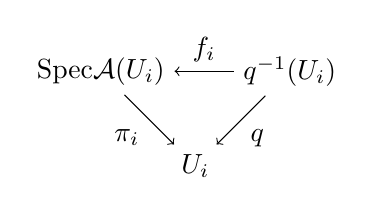
\begin{tikzpicture}[auto,->]
    \node (a) at (0,1.2) {${\rm Spec}{\cal{A}}(U_i)$}; \node (x) at (2.4,1.2) {$q^{-1}(U_i)$};
    \node (b) at (1.2,0) {$U_i$};
    \draw (x) -- node[swap] {$f_i$} (a);

    \draw (a) -- node[swap] {$\pi_i$} (b);
    \draw (x) -- node {$q$} (b);
  \end{tikzpicture}
\]
により$S$-schemeの射$f_i$ができる.$\cal{A}$がq-coh.であることを使うとこれらの$f_i$は貼り合って$S$-schemeの射$f:Y \to {\rm Spec}{\cal{A}}$を定めることがわかる.これがinverseを与えることが計算により確かめられる.自然性は明らか.
\end{proof}
\begin{rem}
  {\rm Thm.\ref{thm:univ}}と米田の補題により,${\rm Spec}{\cal{A}}$は$S$のaffine open covering $(U_i)_i$の取り方によらず定まる.特に$S={\rm SpecR}$がaffine scheme,$R\to A$が$R$代数で${\cal{A}}={\tilde A}$の時
  \[
    {\rm Spec}{\cal{A}}={\rm Spec}A
  \]
  である.
\end{rem}
\begin{ex}[affine $n$-space]
  $S$をschemeとする.q-coh. ${\cal{O}}_S$-algebra ${\cal{O}}_S[t_1,\dots ,t_n]$に対し
  \[
  \mathbb{A}^n_S={\rm Spec}{{\cal{O}}_S[t_1,\dots ,t_n]}
  \]
  と定め,affine $n$-space over $S$という.
\end{ex}



\section{{\it relative spectrum}と表現可能関手}
この章では,relative spectrumをある関手のrepresenting objectとして特徴付ける(\cite{stacks_project}も参照).またそれを利用したfiber productの計算の一例を挙げる.
\begin{defi}\label{thm:functor_F}
  scheme $S$とq-coh. ${\cal{O}}_S$-algebra $\cal{A}$に対し関手$F=F_{(S,{\cal{A}})}:{\bf Sch}^{op} \to {\bf Set}$を,対象については
  \[
    Y \longmapsto F(Y)=\{(q,\varphi)|\mbox{$q:Y \to S$はschemeの射,$\varphi:{\cal{A}} \to q_*{\cal{O}}_Y$は${\cal{O}}_S$-algebraの射}\}
  \]
  によって,射については自然な対応によって定める.
\end{defi}
\begin{thm}\label{thm:rep}
  ${\rm Spec}{\cal{A}}$は$F$のrepresenting objectである.すなわち関手の同型
  \[
    F \cong {\rm Hom}_{\bf Sch}(-,{\rm Spec}{\cal{A}})
  \]
  がある.
\end{thm}
\begin{proof}
  $Y$をschemeとする.$f \in {\rm Hom}_{\bf Sch}(Y,{\rm Spec}{\cal{A}})$とし,$f^{\flat}:{\cal{O}}_{{\rm Spec}{\cal{A}}} \to f_*{\cal{O}}_Y}$を$f$によるsheafの射とする.このとき
  \[
    f \longmapsto (q:Y \xrightarrow{f} {\rm Spec}{\cal{A}} \xrightarrow{\pi} S,\hspace{10pt} \varphi:{\cal{A}} \xrightarrow{\sim} \pi_*{\cal{O}}_{{\rm Spec}{\cal{A}}} \xrightarrow{\pi_*f^{\flat}} q_*{\cal{O}}_Y)
  \]
  により写像${\rm Hom}_{\bf Sch}(Y,{\rm Spec}{\cal{A}}) \to F(Y)$を定める.
  また,$(q.\varphi) \in F(Y)$をThm.\ref{thm:univ}によって$\varphi$に対応する射$f:Y \to {\rm Spec}{\cal{A}}$に送ることにより写像$F(Y) \to {\rm Hom}_{\bf Sch}(Y,{\rm Spec}{\cal{A}})$を定める.これらが互いにinverseであることがThm.\ref{thm:univ}によりわかる.自然性も簡単に確かめられる.
\end{proof}
\begin{prop}\label{thm:pullback}
  $S,S'$をscheme,$g:S' \to S$をschemeの射とし,$\cal{A}$をq-coh. ${\cal{O}}_S$-algebra,${\cal{A'}}=g^*{\cal{A}}$とする(これは{\rm Cor.\ref{thm:invese_q-coh.}}によりq-coh. ${\cal{O}}_{S'}$-algebraである).また$F':{\bf Sch}^{op} \to {\bf Set}$を$(S',{\caL{A'}})$に対応する{\rm Def.\ref{thm:functor_F}}の関手とする.このとき図式
  \[
    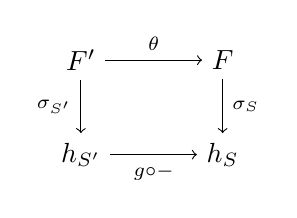
\begin{tikzpicture}[auto,->]
      \node (a) at (0,1.2) {$F'$}; \node (x) at (1.8,1.2) {$F$};
      \node (b) at (0,0) {$h_{S'}$}; \node (y) at (1.8,0) {$h_{S}$};
      \draw (a) -- node {$\scriptstyle \theta$} (x);
      \draw (x) -- node {$\scriptstyle \sigma_{S}$} (y);
      \draw (a) -- node[swap] {$\scriptstyle \sigma_{S'}$} (b);
      \draw (b) -- node[swap] {$\scriptstyle g \circ -$} (y);
    \end{tikzpicture}
  \]
  はpullback (fiber product)である.

  ただし$h_{S}={\rm Hom}_{\bf Sch}(-,S)$は$S$の米田埋め込みによる像,$\theta$は
  \[
    \theta(Y):F'(Y) \longrightarrow F(Y), \hspace{15pt}(q',\varphi') \longmapsto (g \circ q',\varphi')
  \]
  により定まる自然変換,$\sigma_{S}$は第一成分への射影
  \[
    \sigma_S(Y):F(Y)\longrightarrow{\rm Hom}_{\bf Sch}(Y,S)
  \]
  により定まる自然変換である.
\end{prop}
\begin{proof}
  ${\bf Set}$は完備だから,全てのscheme $Y$に対して図式
  \[
    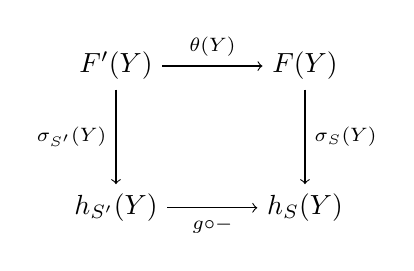
\begin{tikzpicture}[auto,->]
      \node (a) at (0,1.8) {$F'(Y)$}; \node (x) at (2.4,1.8) {$F(Y)$};
      \node (b) at (0,0) {$h_{S'}(Y)$}; \node (y) at (2.4,0) {$h_{S}(Y)$};
      \draw (a) -- node {$\scriptstyle \theta(Y)$} (x);
      \draw (x) -- node {$\scriptstyle \sigma_{S}(Y)$} (y);
      \draw (a) -- node[swap] {$\scriptstyle \sigma_{S'}(Y)$} (b);
      \draw (b) -- node[swap] {$\scriptstyle g \circ -$} (y);
    \end{tikzpicture}
  \]

  がpullbackであることを示せば良い.\footnote{\cite{alg_d},定理10の双対をとる.例14も参照.}

  これは${\bf Set}$におけるpullbackの表示より
  \[
    F(Y)\times_{h_S(Y)} h_{S'}(Y)=\{((q,\varphi),q')\in F(Y)\times h_{S'}(Y)|q=g\circ q'\} \cong F'(Y)
  \]
  であることからわかる.
\end{proof}
\begin{cor}
  $S,S'$をscheme,$g:S' \to S$をschemeの射とし,$\cal{A}$をq-coh. ${\cal{O}}_S$-algebra,${\cal{A'}}=g^*{\cal{A}}$とする.このとき
  \[
  {\rm Spec}{\cal{A'}}={\rm Spec}{\cal{A}}\times_S S'
  \]
  である.
\end{cor}
\begin{proof}
  Thm.\ref{thm:rep}とProp.\ref{thm:pullback}および米田埋め込みの性質より従う.
\end{proof}
\begin{cor}
  $n$を正整数,$S,S'$をscheme,$g:S' \to S$をschemeの射とする.このとき
  \[
    \mathbb{A}^n_{S'}=\mathbb{A}^n_S \times_S S'
  \]
  である.特に
  \[
    \mathbb{A}^n_S=\mathbb{A}^n_{\mathbb{Z}} \times_{{\rm Spec}{\mathbb{Z}}} S
  \]
  である\footnote{実はこの命題について調べていたところ\cite{stacks_project}を発見し,圏論的な証明に感動してこの記事を書いた.}.

\end{cor}
\begin{proof}
  $g^*{{\cal{O}}_S[t_1,\dots ,t_n]}={{\cal{O}}_{S'}[t_1,\dots ,t_n]}$を示せば良い.$t$によって$n$個の変数$(t_1,\dots,t_n)$をまとめて略記する.

  $U={\rm Spec}B \subset S$,
  $U'={\rm Spec}A \subset g^{-1}(U) \subset S'$をそれぞれaffine openとし,$g:U' \to U$に対応する環の射を$\sigma:B \to A$とする.このときq-coh.とProp.\ref{thm:associated}より
  \[
  (g^*{\cal{O}}_S[t])|_{U'}=g^*({\cal{O}}_S[t]|_U)={\widetilde {B[t] \otimes_B A}}\cong {\widetilde{A[t]}}={\cal{O}}_{S'}[t]|_{U'}
  \]
  である.この同型を貼り合わせれば良い.
\end{proof}

\section{おわりに}
relative spectrumの構成の準備に多くのページを割いてしまいましたが,一番書きたかった米田埋め込みによるfiber productの計算をしっかり書くことができて満足です.そもそもの元ネタは\cite{stacks_project}のThe Stacks project 26.4なのですが,そこでの証明は関手の表現可能性の判定についての大掛かりな準備を元にしたものだったので,この記事ではThm.\ref{thm:univ}を軸にした証明をつけています.他にも関連して書きたい話題がいくつかあったのですが,ここの証明の修正に手間取ってしまい時間がないので別の機会に記事にしようと思います.

質問等はtwitter:@alskdjfhg9に連絡お願いします.
\begin{thebibliography}{2}
\bibitem{ハーツホーン} R.ハーツホーン,『代数幾何学1,2,3』,高橋ほか訳,丸善出版,2012.
\bibitem{Gortz} Gortz,Wedhorn, {\sl Algebraic Geometry
Part I: Schemes With Examples and Exercises}, Vieweg+Teubner Verlag, 2010.
\bibitem{Bosch} Siegfried Bosch, {\sl Algebraic Geometry and Commutative Algebra}, Springer, 2013.
\bibitem{stacks_project} {https://stacks.math.columbia.edu/tag/01LQ
}
\bibitem{alg_d}  {http://alg-d.com/math/kan\_extension/limit.pdf}
\end{thebibliography}
\end{document}
